\documentclass[11pt,a4paper,twocolumn]{article}

% === Core Packages ===
\usepackage[margin=2cm]{geometry}
\usepackage[utf8]{inputenc}
\usepackage[T1]{fontenc}
\usepackage{times}
\usepackage{amsmath,amssymb}
\usepackage{graphicx}
\usepackage{booktabs}
\usepackage{float}
\usepackage{enumitem}
\usepackage{tikz}
\usepackage{pgfplots}
\pgfplotsset{compat=1.18}
\usetikzlibrary{arrows.meta,shapes.geometric,positioning,calc,decorations.markings,fit,backgrounds}

% === Citation (IEEE style) ===
\usepackage[numbers,sort&compress]{natbib}
\bibliographystyle{IEEEtranN}

% === Hyperref ===
\usepackage[hidelinks]{hyperref}
\usepackage{xurl}

% === Settings ===
\setlength{\parindent}{1em}
\setlength{\parskip}{0.3em}

% === PDF metadata ===
\hypersetup{
  pdftitle={Rrjeti i Decentralizuar i Reputacionit: Një Kornizë për Organizimin Natyror Shoqëror},
  pdfauthor={Pavel Kudrna},
  pdfsubject={Personix — a decentralized reputation network},
  pdfkeywords={Personix, decentralized reputation, reputation social network,
    decentralized identifiers, DID, meritocracy, censorship resistance},
}

% === Title ===
\title{\textbf{Rrjeti i Decentralizuar i Reputacionit:\\Një Kornizë për Organizimin Natyror Shoqëror}}
\author{Pavel Kudrna\\Personix Project --- \url{https://personix.org}\\Prague, Czechia\\Draft v1 --- March 2026}
\date{}

\begin{document}
\maketitle

% ============================================================
% ABSTRACT
% ============================================================
\begin{abstract}
Ndjenja e drejtësisë---bindja se të gabuarat rregullohen dhe merita shpërblehet---është forca kohezive më e fortë e shoqërisë. Kur institucionet e centralizuara të qeverisjes nuk mund ta ofrojnë këtë ndjenjë sepse kostoja e zbatimit të një të drejte tejkalon vlerën e vetë të drejtës, kohezioni shoqëror gërryhet. Strukturat aktuale institucionale dështojnë të zgjidhin një klasë të konsiderueshme mosmarrëveshjesh në po të njëjtën mënyrë sistematike sikurse planifikimi qendror dështon në shpërndarjen e burimeve: përmes asimetrisë së informacionit, mungesës së cikleve të kthimit të informacionit dhe shkëputjes së vendimmarrësve nga pasojat e vendimeve të tyre. Ky punim paraqet një Rrjet Shoqëror të Reputacionit (RSN): një shtresë komunikimi të decentralizuar, të pakorruptueshme dhe rezistente ndaj censurës, e ndërtuar mbi Identifikuesit e Decentralizuar (DID), e cila u mundëson pjesëmarrësve pseudonimë të publikojnë, verifikojnë dhe konsumojnë informacion reputacioni për sjelljen në botën reale. Mekanizmi themelor mbështetet në tri parime dizajni: (1)~një strukturë kostoje asimetrike ku leximi i të dhënave të reputacionit është i lirë por shkrimi kërkon përpjekje të verifikueshme; (2)~një protokoll jodeterminist të përzgjedhjes së verifikuesit të bazuar në hashimin konsistent, i cili çmon pretendimet radikale përmes kostove në rritje të përsëritjeve; dhe (3)~një model autoriteti reputacioni të drejtuar nga tregu ku verifikuesit privatë vënë në rrezik reputacionin e tyre të akumuluar mbi saktësinë e pretendimeve që miratojnë. Arkitektura që rezulton prodhon meritokraci emergjente pa koordinim qendror dhe mundëson një rrugë migrimi graduale dhe të kthyeshme nga sistemet ekzistuese të administruara nga shteti.
\end{abstract}

% ============================================================
% 1. INTRODUCTION
% ============================================================
\section{Hyrje}

\subsection{Problemi i Besimit të Centralizuar}

Qeverisja moderne mbështetet mbi një supozim themelor: se institucionet e centralizuara mund të ndërmjetësojnë besimin mes të panjohurve në shkallë të gjerë. Gjykatat gjykojnë mosmarrëveshjet. Regjistrat certifikojnë pronësinë. Organet rregullatore zbatojnë standardet. Këto institucione u projektuan në një epokë kur informacioni ishte i pakët, komunikimi ishte i ngadaltë dhe delegimi i autoritetit tek një organ qendror ishte mekanizmi i vetëm i realizueshëm i koordinimit. Megjithatë, qeverisja e centralizuar dështon për të njëjtat arsye strukturore si planifikimi qendror: asimetria e informacionit, mungesa e cikleve të kthimit të informacionit dhe shkëputja e vendimmarrësve nga pasojat e vendimeve të tyre.

Supozimi dështon, për shembull, kur kostoja e ndërmjetësimit institucional tejkalon vlerën e mosmarrëveshjes. Merrni parasysh një qiramarrës i cili zbulon se banesa e tij me qira i mungon një certifikatë sigurie elektrike të kërkuar ligjërisht---një gjendje që paraqet rrezik të menjëhershëm për jetën. E drejta ligjore e qiramarrësit për t'u tërhequr nga kontrata është e paqartësishme. Megjithatë kostoja e zbatimit të asaj të drejte përmes sistemit gjyqësor tejkalon vlerën monetare të depozitës dhe dëmeve që i detyrohen, madje edhe duke përfshirë kompensimin e mundshëm ligjor~\cite{czcourtfees}. Përgjigja racionale është të absorbosh humbjen dhe të largohesh.

Ky nuk është një rast kufitar patologjik. Është përvoja e paracaktuar për një klasë të konsiderueshme mosmarrëveshjesh në të cilat dëmi është real por interesat monetare bien nën pragun në të cilin zbatimi institucional bëhet ekonomikisht racional. Rezultati është një sistem që strukturalisht favorizon aktorët e këqij: ata që dëmtojnë të tjerët në vëllime nën këtë prag mund të veprojnë me pandëshkueshmëri, sepse kostoja e kërkimit të drejtësisë bie mbi palën e dëmtuar.

Shembulli i mësipërm merret nga mjedisi ligjor i autorit---sistemi çek i së drejtës civile. Në traditat e tjera ligjore---e drejta e zakonshme e bazuar në precedent, e drejta zakonore, sistemet e përziera---drejtësia dështon në mënyra të ndryshme dhe në shkallë të ndryshme, në varësi të specifikave kulturore dhe procedurale të juridiksionit. Lexuesit ka të ngjarë të njohin shembuj ekuivalentë nga konteksti i tyre. Ajo që është strukturalisht universale është modeli: mosmarrëveshjet vlera e të cilave bie nën pragun e zbatimit ekonomikisht racional përfundojnë me humbjen që absorbohet nga pala e dëmtuar. RSN nuk premton drejtësi të përsosur---ai thjesht redukton avantazhin strukturor që gëzojnë aktorët e këqij kur zbatimi institucional është joekonomik.

\subsection{Pse Zgjidhjet Ekzistuese Nuk Mjaftojnë}

\textbf{Kornizat e Identitetit të Decentralizuar (DID)}~\cite{did2022} ofrojnë mekanizma kriptografikë për menaxhimin e identitetit vetësovran por përqendrohen kryesisht në verifikimin e identitetit pa trajtuar çështjen më të gjerë të reputacionit të sjelljes.

\textbf{Tokenat e Lidhur me Shpirtin (SBT)}~\cite{weyl2022} kapin njohurinë se reputacioni është i patransferueshëm por mbështeten në infrastrukturën blockchain me kufizime shkallëzueshmërie dhe nuk trajtojnë stimujt ekonomikë që qeverisin hyrjen e informacionit. Konceptet e ngjashme si tokenat e meritës (p.sh., Liberland) ndajnë një filozofi të ngjashme por mbeten të lidhura me korniza specifike juridiksionale.

\textbf{Organizatat Autonome të Decentralizuara (DAO)}~\cite{buterin2014} zbatojnë qeverisjen përmes kontratave inteligjente por riprodhojnë dinamika plutokratike ku ndikimi është proporcional me kapitalin. Votimi kuadratik~\cite{buterin2019} e zbut këtë pjesërisht por kufizon miratimin praktik. DAO-t përballen gjithashtu me \emph{problemin themelor të orakullit}: kontratat inteligjente nuk mund të verifikojnë me besueshmëri gjendjet e botës reale pa një burim të jashtëm të besuar, dhe ky problem nuk ka zgjidhje të përgjithshme brenda arkitekturës blockchain.

Asnjë sistem ekzistues nuk kombinon decentralizimin, rezistencën ndaj censurës, pseudonimitetin, koston e verifikueshme të hyrjes dhe konsensusin emergjent.

\subsection{Kontributet}

Ky punim jep kontributet e mëposhtme:
\begin{enumerate}[nosep]
\item Përkufizimin e \textbf{Rrjetit Shoqëror të Reputacionit (RSN)}, një protokoll të decentralizuar që zgjeron kornizën DID për të mbështetur shkëmbimin dypalësh të reputacionit.
\item Një \textbf{protokoll jodeterminist të përzgjedhjes së verifikuesit} të bazuar në hashimin konsistent~\cite{karger1997}.
\item \textbf{Parimin e Radikalizmit të Kushtueshëm}, i cili çmon pretendimet sipas distancës së tyre nga konsensusi i rrjetit përmes tri kanaleve kostoje që përbëhen mbi njëra-tjetrën.
\item Një \textbf{model Autoriteti të Reputueshëm} me stimuj asimetrikë ku miratimi i rremë kushton në mënyrë katastrofike më shumë se tarifat legjitime.
\item Një \textbf{rrugë migrimi graduale} përmes infrastrukturës fiskale paralele.
\end{enumerate}

% ============================================================
% 2. DESIGN PRINCIPLES
% ============================================================
\section{Parimet e Dizajnit}

Arkitektura e RSN kufizohet nga pesë parime dizajni të panegociueshme.

\textbf{Vazhdimësia dhe Evolucioni.} Sistemi bashkëjeton me institucionet ekzistuese gjatë një periudhe tranzicioni me gjatësi të pacaktuar. Tranzicioni duhet të jetë i kthyeshëm në çdo fazë.

\textbf{Vullnetarizmi dhe Përgjegjësia.} Pjesëmarrja është vullnetare, por vullnetarizmi shoqërohet me përgjegjësi: një pjesëmarrës që merr kontrollin mbi një funksion institucional merr njëkohësisht detyrimet shoqëruese.

\textbf{Diversiteti dhe Neutraliteti Kulturor.} Konsensusi lind nga bashkëveprime dypalëshe, jo nga rregulla të paracaktuara të imponuara nga projektuesit e sistemit.

\textbf{Qëndrueshmëria dhe Rezistenca ndaj Censurës.} Kostoja e censurimit të rrjetit duhet të tejkalojë koston e tolerimit të tij. Vetëm totalitarizmi i plotë---me kosto politike dhe ekonomike shkatërruese---mund ta shtypë sistemin.

\textbf{Konsensusi dhe Zbatimi.} Sistemi përfshin prirjet njerëzore drejt smiritetit, inatit dhe kënaqësisë ndëshkuese si veçori mbajtëse. Sjellja e keqe nuk ndalohet; ajo çmohet.

% ============================================================
% 3. SYSTEM OVERVIEW
% ============================================================
\section{Përmbledhje e Sistemit}

\subsection{Rrjeti Shoqëror i Reputacionit}

RSN është një shtresë komunikimi e decentralizuar, nga bashkëmoshatarë tek bashkëmoshatarë në të cilën pjesëmarrësit shkëmbejnë informacion të verifikueshëm për sjelljen në botën reale. Veçoritë e tij përcaktuese janë: infrastrukturë e decentralizuar dhe e pacensurueshme; pjesëmarrje pseudonime përmes DID-ve; strukturë kostoje asimetrike (leximi është i lirë, shkrimi është i kushtueshëm); verifikueshmëri kriptografike; dhe \textbf{mbështetje standardesh}---formate të lexueshme nga makina për informacionin e përhapur nëpër rrjet, për shërbimet e ofruara nga autoritetet (përbërja e pretendimit, miratimi, shërbimi i dëshmitarit) dhe për formatin e politikës duke përfshirë rregullat për vlerësimin e reputacionit të palës tjetër dhe vlerësimin e rrezikut të mospërputhjes së politikës (mes sjelljes së deklaruar dhe asaj aktuale).

\subsection{Komponentët Arkitekturorë}

RSN përbëhet nga katër komponentë kryesorë (Fig.~\ref{fig:architecture}):
\begin{enumerate}[nosep]
\item \textbf{Shtresa DID.} Identitetet e pjesëmarrësve me rregulla të deklaruara, metadata reputacioni dhe rrugëzim rrjeti.
\item \textbf{Protokolli i Pretendimit.} Format i strukturuar për publikimin e pohimeve për ngjarjet e botës reale.
\item \textbf{Rrjeti i Verifikimit.} Protokoll i decentralizuar për caktimin e verifikuesve duke përdorur hashimin konsistent.
\item \textbf{Shtresa e Grumbullimit të Reputacionit.} Shërbime që prodhojnë përmbledhje reputacioni të lexueshme nga njeriu.
\end{enumerate}

\begin{figure}[ht]
\centering
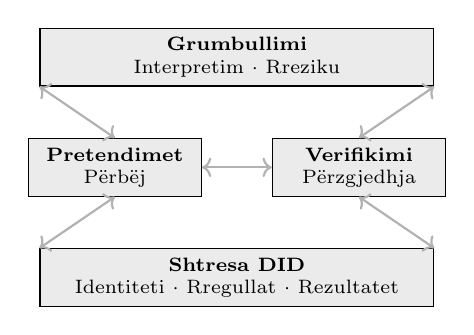
\begin{tikzpicture}[
    layer/.style={draw, minimum height=0.7cm, align=center, font=\scriptsize, fill=black!8},
    arr/.style={<->, thick, gray!60}
]
\node[layer, minimum width=5cm] (agg) at (0,2.8) {\textbf{Grumbullimi}\\Interpretim\ $\cdot$ Rreziku};
\node[layer, minimum width=2.2cm] (claim) at (-1.55,1.4) {\textbf{Pretendimet}\\Përbëj};
\node[layer, minimum width=2.2cm] (verif) at (1.55,1.4) {\textbf{Verifikimi}\\Përzgjedhja};
\node[layer, minimum width=5cm] (did) at (0,0) {\textbf{Shtresa DID}\\Identiteti $\cdot$ Rregullat $\cdot$ Rezultatet};

\draw[arr] (agg.south west) -- (claim.north);
\draw[arr] (agg.south east) -- (verif.north);
\draw[arr] (claim.east) -- (verif.west);
\draw[arr] (claim.south) -- (did.north west);
\draw[arr] (verif.south) -- (did.north east);
\end{tikzpicture}
\caption{Arkitektura katërshtresore e RSN.}
\label{fig:architecture}
\end{figure}

\subsection{Rolet e Pjesëmarrësve}

Një transaksion verifikimi përfshin deri në gjashtë role të dallueshme DID (Fig.~\ref{fig:roles}): \textbf{Lëshuesi} ($DID_I$, krijon dhe paraqet pretendimin), \textbf{Subjekti} ($DID_S$, DID-i për të cilin bëhet pretendimi---mund të përkojë me Lëshuesin), \textbf{Autoriteti} ($DID_A$, miraton pretendimin kundrejt një tarife; mund të ofrojë gjithashtu shërbime dëshmitari---\emph{opsional}), \textbf{Dëshmitari} ($DID_{W_{1..n}}$, monitorues inkognito i ndershmërisë së verifikuesit përmes kodeve të sfidës---\emph{opsional}), \textbf{Verifikuesi} ($DID_V$, i përzgjedhur algoritmikisht për të publikuar pretendimin) dhe \textbf{RSN} (rrjeti ku publikohen pretendimet e verifikuara). Çdo rol mund t'i delegohet një DID-i tjetër (Seksioni~7.4). Një Autoritet zakonisht bashkon miratimin me shërbimet e dëshmitarit, por dy funksionet janë logjikisht të pavarura.

\begin{figure}[ht]
\centering
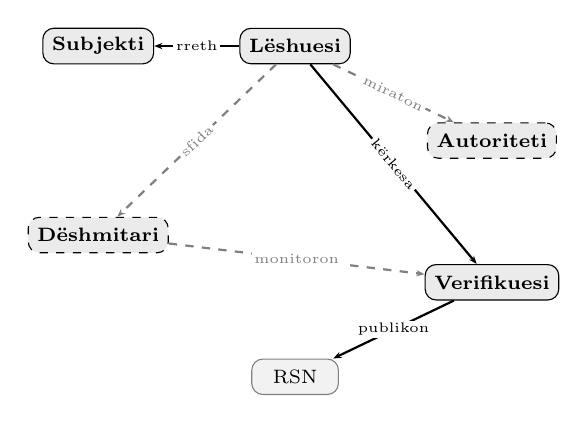
\begin{tikzpicture}[
    role/.style={draw, rounded corners, minimum width=1.1cm, minimum height=0.45cm, align=center, font=\scriptsize, fill=black!8},
    opt/.style={draw, rounded corners, minimum width=1.1cm, minimum height=0.45cm, align=center, font=\scriptsize, fill=black!8, dashed},
    arr/.style={-{Stealth[length=3pt]}, thick},
    oarr/.style={-{Stealth[length=3pt]}, thick, dashed, gray},
    lbl/.style={font=\tiny, fill=white, inner sep=1pt}
]
\node[role] (I) at (0,2.4) {\textbf{Lëshuesi}};
\node[role] (S) at (-2.5,2.4) {\textbf{Subjekti}};
\node[opt] (A) at (2.5,1.2) {\textbf{Autoriteti}};
\node[opt] (W) at (-2.5,0) {\textbf{Dëshmitari}};
\node[role] (V) at (2.5,-0.6) {\textbf{Verifikuesi}};
\node[role, fill=black!5, draw=gray] (N) at (0,-1.8) {RSN};

\draw[arr] (I) -- node[lbl] {rreth} (S);
\draw[oarr] (I) -- node[lbl,sloped] {miraton} (A);
\draw[oarr] (I) -- node[lbl,sloped] {sfida} (W);
\draw[arr] (I) -- node[lbl,sloped] {kërkesa} (V);
\draw[oarr] (W) -- node[lbl] {monitoron} (V);
\draw[arr] (V) -- node[lbl] {publikon} (N);
\end{tikzpicture}
\caption{Rolet DID në një transaksion verifikimi. Me vija të ndërprera = opsionale (Autoriteti, Dëshmitari).}
\label{fig:roles}
\end{figure}

\subsection{Pakorruptueshmëria: Katër Forcat}

Pakorruptueshmëria e RSN nuk lind nga një mekanizëm i vetëm por nga katër forca të njëkohshme. Asnjëra nuk mjafton më vete; vetëm kombinimi i tyre e bën një përpjekje për korrupsion ekonomikisht irracionale.

\textbf{Objektivi i paparashikueshëm.} Verifikuesi për çdo pretendim përzgjidhet jodeterministikisht përmes hashimit konsistent (Seksioni~5.3). Një sulmues nuk mund të synojë paraprakisht një verifikues specifik për ryshfet, sepse identiteti i verifikuesit është funksion i përmbajtjes së pretendimit dhe përsëritjeve të mëparshme, jo i zgjedhjes së lëshuesit.

\textbf{Leva e reputacionit---ngrihet ngadalë, bie shpejt.} Reputacioni mund të fitohet vetëm në mënyrë graduale, përmes sjelljes konsistente të vazhdueshme. Ai megjithatë mund të humbet në mënyrë katastrofike me një miratim të vetëm mashtrues (Seksioni~6.2). Kjo asimetri do të thotë se vite reputacioni i akumuluar mund të shkatërrohet nga një miratim i vetëm i pandershëm; strategjia optimale mbetet të hidhen poshtë pretendimet e dyshimta.

\textbf{Premtimi publik.} Çdo Mbajtës DID deklaron publikisht politikën e tij---një grup rregullash të lexueshme nga makina të cilat zotohet t'i ndjekë. Ndryshimi mes deklaratës dhe sjelljes aktuale është i zbulueshëm dhe çmohet si një shkelje reputacioni më e rëndë se vetë shkelja themelore (Seksioni~7.3). Hipokrizia është pra më e kushtueshme se pandershmëria e drejtpërdrejtë.

\textbf{Asimetria e kostos së sulmit të rrjetit.} Kostoja e censurimit ose destabilizimit të rrjetit rritet në mënyrë jolineare me madhësinë dhe dendësinë e rrjetit, ndërsa kostoja e tolerimit të tij mbetet konstante. Që censura të japë fryte, një aktor i centralizuar do të duhej ta zbatonte atë në të gjithë rrjetin---duke kërkuar masa joproporcionale me çdo përfitim të konceptueshëm (Seksioni~10).

% ============================================================
% 4. DECENTRALIZED IDENTITY MODEL
% ============================================================
\section{Modeli i Identitetit të Decentralizuar}

\subsection{DID me Veti të Veçanta}

RSN zgjeron specifikimin W3C DID Core~\cite{did2022} me: \textbf{Rregulla të Deklaruara} (zotime sjelljeje të lexueshme nga makina), \textbf{Metadata Reputacioni} (rezultat i grumbulluar sjelljeje) dhe \textbf{Rrugëzim Rrjeti} (portë onion e ndryshueshme e ndarë nga pozicioni i qëndrueshëm në unazë).

\subsection{Cikli i Jetës së Pretendimit}

Një Pretendim kalon nëpër gjashtë faza (Fig.~\ref{fig:lifecycle}): përbërja, miratimi opsional nga autoriteti, përzgjedhja e verifikuesit përmes hashimit konsistent, vendimi i verifikimit (pranim ose refuzim me përsëritje), publikimi dhe përditësimi i reputacionit për të gjitha palët.

\begin{figure}[ht]
\centering
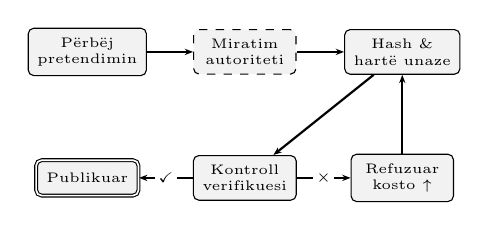
\begin{tikzpicture}[
    stp/.style={draw, rounded corners=2pt, minimum width=1.3cm, minimum height=0.45cm, align=center, font=\tiny, fill=black!5},
    arr/.style={-{Stealth[length=3pt]}, thick},
    lbl/.style={font=\tiny, fill=white, inner sep=1pt}
]
\node[stp] (comp) at (0,0) {Përbëj\\pretendimin};
\node[stp, dashed] (auth) at (2.0,0) {Miratim\\autoriteti};
\node[stp] (hash) at (4.0,0) {Hash \&\\hartë unaze};
\node[stp] (ver) at (2.0,-1.6) {Kontroll\\verifikuesi};
\node[stp, double] (pub) at (0,-1.6) {Publikuar};
\node[stp] (rej) at (4.0,-1.6) {Refuzuar\\kosto $\uparrow$};

\draw[arr] (comp) -- (auth);
\draw[arr] (auth) -- (hash);
\draw[arr] (hash) -- (ver);
\draw[arr] (ver) -- node[lbl] {\checkmark} (pub);
\draw[arr] (ver) -- node[lbl] {$\times$} (rej);
\draw[arr] (rej) -- ++(0,0.8) -| (hash);
\end{tikzpicture}
\caption{Cikli i jetës së pretendimit me lak përsëritjeje.}
\label{fig:lifecycle}
\end{figure}

\subsection{Marrëdhënia me W3C DID Core}

Modeli i identitetit të RSN është një superbashkësi e mirëfilltë e specifikimit W3C DID Core~\cite{did2022}. Të gjitha DID-të e RSN janë DID të vlefshme W3C. Zgjerimet specifike të RSN kodohen si veti të dokumentit DID të përcaktuara në një specifikim të dedikuar metode DID, të përputhshëm me infrastrukturën ekzistuese si ION~\cite{buchner2021} dhe Ceramic~\cite{ceramic2023}.

% ============================================================
% 5. VERIFICATION AND PROPAGATION
% ============================================================
\section{Verifikimi dhe Përhapja e Informacionit}

\subsection{Kostoja e Hyrjes së Informacionit}

Parimi themelor ekonomik i RSN është asimetria mes leximit dhe shkrimit. Leximi i të dhënave të reputacionit i afrohet kostos margjinale zero për pjesëmarrësit që janë pjesë e rrjetit DID dhe kanë qasje në përpjesëtim me reputacionin e tyre---të sapoardhurit duhet të fitojnë gradualisht qasje më të gjerë (shih anti-parazitizmin). Shkrimi---i kuptuar si materializimi i qëndrueshëm i reputacionit në rrjet, jo si një akt teknik i njëhershëm---kërkon investim kumulativ të verifikueshëm nëpër tri dimensione: \textbf{koha} (vite jete të shpenzuara në sjellje konsistente, zotime të përmbushura dhe marrëdhënie të kultivuara), \textbf{energjia} (përpjekja e investuar në marrëveshje të ndershme, kujdesi për partneritetet dhe besueshmëria afatgjatë) dhe \textbf{paraja} (investimi në emrin e vet---zhvillimi profesional, cilësia e punës së dikujt, riparimi për dëmet e shkaktuara). Reputacioni nuk mund të blihet menjëherë---ai është rezultati i akumulimit gjatë gjithë jetës që sistemi thjesht e bën të dukshëm dhe të transferueshëm nëpër kontekste. Kostot teknike të njëhershme të protokollit (nënshkrimet kriptografike, tarifat e verifikuesit) janë të papërfillshme krahasuar me këtë investim themelor.

\subsection{Grafi Shoqëror dhe Thellësia e Kontakteve}

RSN është thelbësisht një rrjet shoqëror: çdo DID shton kontakte (DID të tjera) që e lejojnë lidhjen. Këto kontakte kanë kontaktet e tyre, e kështu me radhë. Kërkimi algoritmik i verifikuesit vepron brenda një thellësie të konfigurueshme $h$ kontaktesh të lidhura (p.sh., $h=3$: kontaktet e drejtpërdrejta të dikujt, kontaktet e tyre dhe kontaktet e kontakteve). Kjo arkitekturë nuk kërkon një blockchain të vetëm global---ajo favorizon natyrshëm shfaqjen e komuniteteve/grumbujve me mbivendosje në komunitete të tjera. Çdo pjesëmarrës DID duhet të ketë një \textbf{politikë} të publikuar---një grup rregullash të lexueshme nga makina që qeverisin mënyrën se si vlerësohen kërkesat hyrëse. Shkeljet e politikës regjistrohen në rrjet si artefakte negative.

\subsection{Përzgjedhja Algoritmike e Verifikuesit}

Protokolli i verifikimit përdor hashimin konsistent~\cite{karger1997} (Fig.~\ref{fig:verifier}). Verifikimi është një shërbim me pagesë: verifikuesit veprojnë kundrejt një tarife, duke krijuar një treg ku konkurrenca përcakton çmimin, shpejtësinë dhe besueshmërinë.

\textbf{Hapi 1.} Dokumenti i pretendimit bashkohet me rezultatin e hash-it të përsëritjes së mëparshme (ose $\varnothing$ në përsëritjen e parë) dhe hashohet:
\begin{equation}
\text{pos} = f_h(\text{claim} \| \text{prev\_hash})
\label{eq:hash}
\end{equation}

Algoritmi duhet të përfshijë \emph{rrugën e plotë} të të gjitha kërkesave dhe përgjigjeve të mëparshme---jo thjesht një hash të përsëritjes së mëparshme. Përgjigja e plotë e çdo verifikuesi (pranimi, refuzimi, çmimi i cituar, arsyeja) i shtohet dokumentit në rritje, e verifikueshme përmes nënshkrimeve kriptografike në çdo hap.

\textbf{Hapi 2.} Hash-i hartohet në $N$ pozicione në unazën e hashit konsistent, të shpërndara njëtrajtësisht (p.sh., për $N=4$: $+0^{\circ}, +90^{\circ}, +180^{\circ}, +270^{\circ}$). Nga çdo pozicion, një kërkim në drejtim orar përzgjedh DID-in më të afërt si kandidat verifikuesi (Fig.~\ref{fig:multipoint}). $N$ është një parametër i ndryshueshëm që mund të varet nga përqindja e DID-ve aktualisht aktive, ora e ditës ose reagueshmëria historike e rrjetit.

\textbf{Hapi 3.} Verifikuesi pranon (publikon, duke vënë në rrezik reputacionin) ose refuzon (duke u kthyer te Hapi~1 me hash-in e refuzimit). Kur një nyje nuk përgjigjet pavarësisht se ka deklaruar statusin online, kërkesa e radhës duhet të përfshijë të gjitha përgjigjet nga të gjithë $N$ kandidatët e mëparshëm të verifikuesit.

\textbf{Anti-parazitizmi.} DID-të objektiv mund të vendosin tarifa ose kufizime qasjeje për pyetësimet nga DID të reja me pak reputacion. Ky mekanizëm i shkallëzuar (jo binar) i detyron të sapoardhurit të ndërtojnë reputacion përmes aktivitetit të vërtetë përpara se të konsumojnë lirisht të dhënat e të tjerëve.

\begin{figure}[ht]
\centering
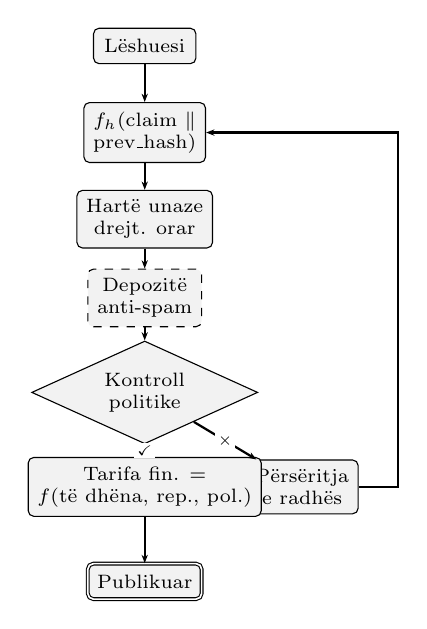
\begin{tikzpicture}[
    box/.style={draw, rounded corners=2pt, minimum width=1.3cm, minimum height=0.45cm, align=center, font=\scriptsize, fill=black!5},
    dec/.style={draw, diamond, aspect=2.2, minimum width=0.9cm, align=center, font=\scriptsize, fill=black!5},
    arr/.style={-{Stealth[length=3pt]}, thick},
    lbl/.style={font=\tiny, fill=white, inner sep=1pt}
]
\node[box] (iss) at (0,0) {Lëshuesi};
\node[box] (hash) at (0,-1.1) {$f_h$(claim $\|$\\prev\_hash)};
\node[box] (ring) at (0,-2.2) {Hartë unaze\\drejt. orar};
\node[box, dashed] (spam) at (0,-3.2) {Depozitë\\anti-spam};
\node[dec] (check) at (0,-4.4) {Kontroll\\politike};
\node[box] (rej) at (2,-5.6) {Përsëritja\\e radhës};
\node[box] (fee) at (0,-5.6) {Tarifa fin. =\\$f$(të dhëna, rep., pol.)};
\node[box, double] (pub) at (0,-6.8) {Publikuar};

\draw[arr] (iss) -- (hash);
\draw[arr] (hash) -- (ring);
\draw[arr] (ring) -- (spam);
\draw[arr] (spam) -- (check);
\draw[arr] (check) -- node[lbl] {$\times$} (rej);
\draw[arr] (check) -- node[lbl] {\checkmark} (fee);
\draw[arr] (fee) -- (pub);
\draw[arr] (rej.east) -- ++(0.5,0) |- (hash.east);
\end{tikzpicture}
\caption{Protokolli i përzgjedhjes së verifikuesit. Depozita anti-spam është opsionale dhe mund të rimbursohet. Tarifa përfundimtare paguhet vetëm pas pranimit.}
\label{fig:verifier}
\end{figure}

Çdo refuzim i shton pretendimit përgjigjen e plotë të verifikuesit (duke përfshirë arsyet dhe kushtet), duke zgjeruar përmbajtjen e tij. Nga dokumenti i zgjeruar, një hash i ri llogaritet jodeterministikisht, duke u hartuar në një pozicion tjetër të unazës dhe duke përzgjedhur një verifikues tjetër. Dokumentimi i rrugës së plotë është i detyrueshëm---lëshuesi nuk mund të parashikojë ose ndikojë verifikuesin e radhës. Nëse një verifikues shpërfill një kërkesë pavarësisht një politike të deklaruar të përputhshme, dëshmitarët (nëse janë të pranishëm) e regjistrojnë këtë, dhe lëshuesi mund të bashkëngjisë provat e dëshmitarit gjatë publikimit përfundimtar.

\begin{figure}[ht]
\centering
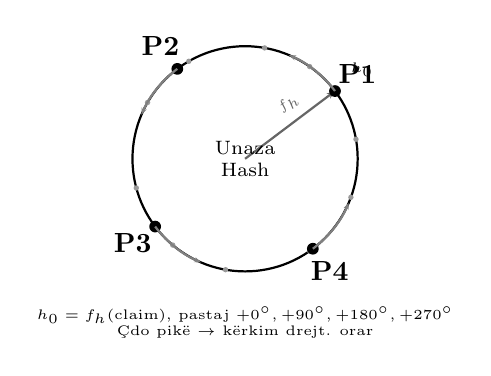
\begin{tikzpicture}[scale=0.65]
% Ring
\draw[thick] (0,0) circle (2.2cm);
% DID nodes on ring
\foreach \a in {10,55,80,120,150,195,230,260,305,340} {
  \fill[black!40] (\a:2.2) circle (1.5pt);
}
% Hash offset arrow pointing to initial position
\draw[-{Stealth[length=3pt]}, thick, black!60] (0,0) -- node[font=\tiny,above,sloped,pos=0.6] {$f_h$} (37:2.2);
\fill[black] (37:2.2) circle (2pt);
\node[font=\tiny,anchor=south west] at (37:2.35) {$h_0$};
% N=4 points offset from h0 by +0, +90, +180, +270
\foreach \offset/\l in {0/P1,90/P2,180/P3,270/P4} {
  \pgfmathsetmacro{\ang}{37+\offset}
  \node[fill=black, circle, inner sep=1.5pt] (p\offset) at (\ang:2.2) {};
  \node[font=\tiny,font=\bfseries] at (\ang:2.75) {\l};
  % clockwise search arc
  \draw[-{Stealth[length=2.5pt]}, thick, gray] (\ang:2.2) arc (\ang:\ang+30:2.2);
}
\node[font=\scriptsize, align=center] at (0,0) {Unaza\\Hash};
\node[font=\tiny, align=center] at (0,-3.2) {$h_0 = f_h(\text{claim})$, pastaj $+0^{\circ},+90^{\circ},+180^{\circ},+270^{\circ}$\\Çdo pikë $\rightarrow$ kërkim drejt. orar};
\end{tikzpicture}
\caption{Përzgjedhja shumëpikëshe ($N{=}4$). Hash-i $h_0$ vendos zhvendosjen; 4 pika të shpërndara njëtrajtësisht nga $h_0$.}
\label{fig:multipoint}
\end{figure}

\subsection{Protokolli i Dëshmitarit}

Roli i \textbf{Dëshmitarit} ofron llogaridhënie inkognito për ndershmërinë e verifikuesit përmes një protokolli kriptografik të kodit të sfidës:

\textbf{Hapi D1.} Kërkuesi nënshkruan kërkesën e verifikimit dhe ia dërgon $N_w$ dëshmitarëve---kontakte nga rrjeti shoqëror i kërkuesit, ose ofrues të specializuar të shërbimit të dëshmitarit që veprojnë kundrejt një tarife.

\textbf{Hapi D2.} Çdo dëshmitar $w_i$ nënshkruan të gjithë kërkesën e nënshkruar, ruan nënshkrimin origjinal $\sigma_i$ dhe llogarit një kod sfide $c_i = h(\sigma_i)$. Kodi i sfidës i shtohet kërkesës.

\textbf{Hapi D3.} Kërkesa, që tani mbart $N_w$ kode sfide, i dërgohet verifikuesit. Verifikuesi vëzhgon kodet por \emph{nuk mund të përcaktojë} kush janë dëshmitarët ose nëse kodet u korrespondojnë nënshkrimeve reale.

\textbf{Hapi D4 (verifikues i ndershëm).} Nëse verifikuesi përgjigjet sipas politikës së tij të deklaruar, kodet e sfidës mbeten të errëta. Dëshmitarët nuk zbulohen kurrë. Nuk publikohen të dhëna shtesë.

\textbf{Hapi D5 (shkelje politike).} Nëse verifikuesi shkel politikën e tij (shpërfill kërkesën, përgjigjet në mënyrë të mospërputhshme), kërkuesi zotëron nënshkrimet origjinale të dëshmitarëve $\sigma_i$. Këto mund të publikohen si të dhëna shoqëruese: kushdo mund të verifikojë $c_i = h(\sigma_i)$, duke vërtetuar se dëshmitari ishte i pranishëm. Kërkuesi mund të publikojë në mënyrë të pavarur---verifikuesi tashmë i nënshkroi kodet e sfidës në përgjigjen e tij.

\textbf{Vetia e bllofit.} Kërkuesi mund të zëvendësojë vlera të rastësishme për disa ose të gjitha kodet e sfidës. Verifikuesi nuk mund të dallojë kodet e vërteta (të mbështetura nga autoritete me reputacion të lartë) nga zhurma. Kjo \emph{pasiguri} është mekanizmi zbatues: çdo kërkesë mbart rrezikun se një autoritet i respektuar po shikon inkognito. Kostoja e mbajtjes së këtij presioni është pothuajse zero (gjenerimi i numrave të rastësishëm), ndërsa kostoja e mundshme e pandershmërisë për verifikuesin është katastrofike. Sjellja e ndershme stimulohet edhe në mungesë të dëshmitarëve realë.

\textbf{Autoriteti si dëshmitar.} Një Autoritet që miraton një pretendim mund të bashkojë shërbimet e dëshmitarit: ``Unë miratoj pretendimin tënd dhe shërbej si dëshmitar inkognito gjatë verifikimit.'' Ky është një model biznesi natyror---Autoriteti tashmë e ka kontekstin. Megjithatë, dy rolet janë logjikisht të pavarura.

\subsection{Parimi i Radikalizmit të Kushtueshëm}

Tri kanale kostoje përbëhen njëkohësisht (Fig.~\ref{fig:radicalism}):

\textbf{Kanali 1: Kostoja e Përsëritjes.} Çdo refuzim detyron një përsëritje të re duke konsumuar kohë dhe burime. Rritje lineare.

\textbf{Kanali 2: Fryrja e Dokumentit.} Çdo përsëritje i shton pretendimit përgjigjen e plotë të verifikuesit. Rritja është lineare, por me një zhvendosje bazë: ngarkesa fillestare (përmbajtja e pretendimit, miratimi i autoritetit, nënshkrimet kriptografike) tashmë ka madhësi jotriviale $B_0$. Madhësia totale pas $k$ përsëritjesh: $S(k) = B_0 + k \cdot \Delta$, ku $\Delta$ është madhësia mesatare e përgjigjes.

\textbf{Kanali 3: Primi i Rrezikut të Verifikuesit.} Rreziku është subjektiv. Verifikuesi vlerëson nëse politikat e deklaruara të DID-it kërkues bien ndesh me interesat komerciale, shoqërore ose politike të vetë verifikuesit. Primi mund të përshkallëzohet eksponencialisht me distancën e perceptuar nga ``ideali'' i verifikuesit: $P(d) = \alpha \cdot e^{\beta d}$, ku $d$ është metrika subjektive e distancës e verifikuesit. Përtej një kufiri personal të ndaluar, verifikuesi mund të refuzojë plotësisht.

\begin{figure}[ht]
\centering
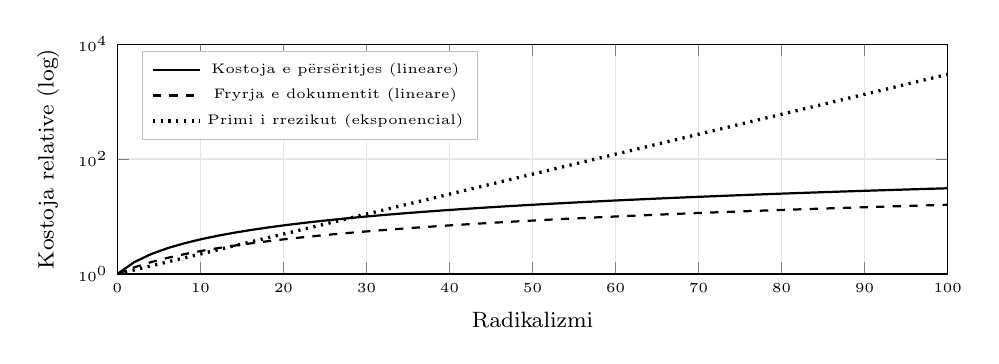
\begin{tikzpicture}
\begin{axis}[
    width=\columnwidth,
    height=4.5cm,
    xlabel={\footnotesize Radikalizmi},
    ylabel={\footnotesize Kostoja relative (log)},
    ymode=log,
    xmin=0, xmax=100,
    ymin=1, ymax=10000,
    grid=major,
    grid style={gray!20},
    legend style={at={(0.03,0.97)},anchor=north west,font=\tiny,draw=gray!50},
    tick label style={font=\tiny},
    label style={font=\footnotesize},
]
\addplot[black, thick, domain=0:100, samples=50] {1 + 0.3*x};
\addlegendentry{Kostoja e përsëritjes (lineare)}
\addplot[black, thick, dashed, domain=0:100, samples=50] {1 + 0.15*x};
\addlegendentry{Fryrja e dokumentit (lineare)}
\addplot[black, thick, dotted, line width=1.2pt, domain=0:100, samples=100] {exp(0.08*x)};
\addlegendentry{Primi i rrezikut (eksponencial)}
\end{axis}
\end{tikzpicture}
\caption{Përshkallëzimi i kostos nëpër tri kanale. Primi i rrezikut dominon në radikalizëm të lartë.}
\label{fig:radicalism}
\end{figure}

Në mënyrë kritike, kjo nuk është censurë. Asnjë pretendim nuk ndalohet. Sistemi çmon rrezikun (Tabela~\ref{tab:costs}).

\begin{table}[ht]
\centering
\caption{Krahasimi i kostos nëpër llojet e pretendimeve.}
\label{tab:costs}
\footnotesize
\begin{tabular}{@{}lcccc@{}}
\toprule
\textbf{Lloji} & \textbf{Përs.} & \textbf{Dok} & \textbf{Tarifa} & \textbf{Total} \\
\midrule
I besueshëm & $k_{\min}$ & $B_0$ & $P_{\min}$ & I ulët \\
I diskutueshëm & $k_{\text{med}}$ & $B_0{+}k\Delta$ & $\alpha e^{\beta d}$ & I moderuar \\
Radikal & $k_{\max}$ & $\gg B_0$ & $\gg P_{\min}$ & Shumë i lartë \\
Mashtrues & $\to\infty$ & --- & --- & I papublikueshëm \\
\bottomrule
\end{tabular}
\end{table}

% ============================================================
% 6. REPUTATION AND RISK
% ============================================================
\section{Reputacioni dhe Vlerësimi i Rrezikut}

\subsection{Modeli i Akumulimit të Reputacionit}

Reputacioni shfaq tri veti: \textbf{akumulim i ngadaltë} (rritje graduale përmes sjelljes konsistente), \textbf{shkatërrim i shpejtë} (një mashtrim i vetëm mund ta reduktojë rezultatin në mënyrë katastrofike) dhe \textbf{vlerësim individual} (çdo palë konsumuese mund të zbatojë funksionin e vet të grumbullimit).

\subsection{Autoritetet e Reputueshme}

Një Autoritet i Reputueshëm shqyrton pretendimet dhe, nëse është i kënaqur, i bashkënënshkruan---duke vënë në rrezik reputacionin e vet (Fig.~\ref{fig:authority}). Asimetria është e qëllimshme: fitimi i reputacionit është i ngadaltë (rritje graduale $+\delta$ për çdo miratim të ndershëm), ndërsa humbja e tij është katastrofike ($-\Delta \gg \delta$ për çdo miratim të rremë; ilustrueshëm, p.sh., $+2\%$ kundrejt $-70\%$). Strategjia optimale është gjithmonë të hidhen poshtë pretendimet e dyshimta. Vlerat specifike të $\delta$ dhe $\Delta$ janë parametra sistemi.

\begin{figure}[ht]
\centering
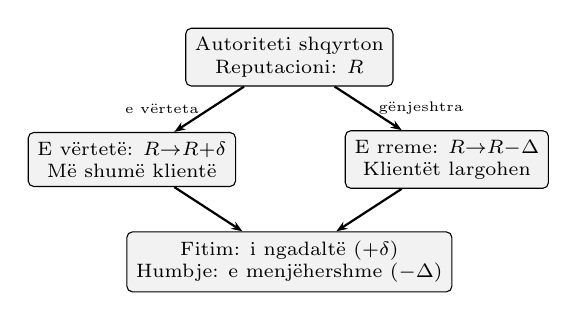
\begin{tikzpicture}[
    box/.style={draw, rounded corners=2pt, minimum width=2cm, minimum height=0.6cm, align=center, font=\scriptsize, fill=black!5},
    arr/.style={-{Stealth[length=4pt]}, thick}
]
\node[box] (exam) at (0,0) {Autoriteti shqyrton\\Reputacioni: $R$};
\node[box] (true) at (-2,-1.3) {E vërtetë: $R{\to}R{+}\delta$\\Më shumë klientë};
\node[box] (false) at (2,-1.3) {E rreme: $R{\to}R{-}\Delta$\\Klientët largohen};
\node[box] (insight) at (0,-2.6) {Fitim: i ngadaltë ($+\delta$)\\Humbje: e menjëhershme ($-\Delta$)};

\draw[arr] (exam) -- node[left,font=\tiny] {e vërteta} (true);
\draw[arr] (exam) -- node[right,font=\tiny] {gënjeshtra} (false);
\draw[arr] (true) -- (insight);
\draw[arr] (false) -- (insight);
\end{tikzpicture}
\caption{Autoriteti i Reputueshëm---stimuj asimetrikë.}
\label{fig:authority}
\end{figure}

\subsection{Reputacioni Shumëdimensional}

Reputacioni nuk është një skalar por një vektor nëpër shumë dimensione: besueshmëria financiare, integriteti personal, kompetenca profesionale, angazhimi qytetar dhe të tjera (Fig.~\ref{fig:reputation-radar}). Ofrues të ndryshëm vlerësimi e projektojnë këtë vektor ndryshe në varësi të kontekstit---një huadhënës i jep përparësi besueshmërisë financiare, një punëdhënës kompetencës profesionale, një fqinj sjelljes qytetare. Nuk ka një rezultat të vetëm ``të saktë'' reputacioni; ka vetëm perspektiva.

\begin{figure}[ht]
\centering
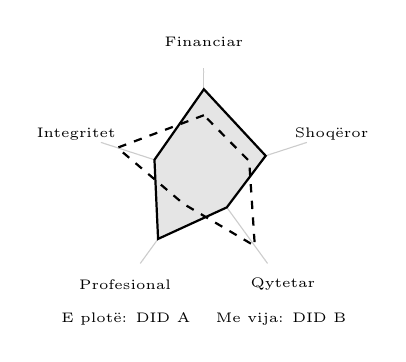
\begin{tikzpicture}[scale=0.55]
\foreach \a/\l in {90/Financiar,162/Integritet,234/Profesional,306/Qytetar,18/Shoqëror} {
  \draw[gray!40] (0,0) -- (\a:2.5);
  \node[font=\tiny, align=center] at (\a:3.1) {\l};
  \foreach \r in {0.8,1.6,2.4} {
    \fill[black!15] (\a:\r) circle (0.5pt);
  }
}
\draw[thick, fill=black!10] (90:2.0) -- (162:1.2) -- (234:1.8) -- (306:0.9) -- (18:1.5) -- cycle;
\draw[thick, dashed] (90:1.4) -- (162:2.1) -- (234:0.8) -- (306:2.0) -- (18:1.1) -- cycle;
\node[font=\tiny] at (0,-3.3) {E plotë: DID A \quad Me vija: DID B};
\end{tikzpicture}
\caption{Vektorët shumëdimensionalë të reputacionit. DID të ndryshme shfaqin profile të ndryshme nëpër dimensione.}
\label{fig:reputation-radar}
\end{figure}

\subsection{Vlerësimi i Demokratizuar i Rrezikut}

RSN e demokratizon vlerësimin sistematik të rrezikut---një aftësi aktualisht e përqendruar në institucionet financiare por e zbatueshme shumë përtej bankingut. Konglomeratet industriale që vlerësojnë besueshmërinë e furnizuesve, kompanitë e sigurimit që çmojnë rrezikun e sjelljes, kujdesi i duhur për bashkimet dhe blerjet, vlerësimi i jetëgjatësisë së pajisjeve në prodhim---kudo që rreziku i palës tjetër kërkon vlerësim, RSN ofron një alternativë të decentralizuar, të drejtuar nga tregu. Një treg shërbimesh interpretimi përkthen të dhëna të papërpunuara shumëdimensionale reputacioni në përmbledhje të veprueshme, duke e bërë vlerësimin e palës tjetër të qasshëm për çdo pjesëmarrës me kosto margjinale.

% ============================================================
% 7. CONSENSUS AND DISPUTE RESOLUTION
% ============================================================
\section{Konsensusi dhe Zgjidhja e Mosmarrëveshjeve}

\subsection{Modeli i Drejtësisë së Decentralizuar}

RSN e riformulon drejtësinë si një problem negocimi dypalësh. Kërcënimi i dëmit të përhershëm dhe të verifikueshëm të reputacionit është një pengues më efektiv se procedurat ligjore që pala e dëmtuar nuk mund t'i përballojë.

\subsection{Konsensusi Emergjent}

Çdo pjesëmarrës mban një prag personal kënaqësie. Konsensusi i grumbulluar i rrjetit lind si mesatarja statistikore e mijëra negocimeve dypalëshe (Fig.~\ref{fig:consensus}). Një përgjigje shumë mbi konsensusin (barbare) është e kushtueshme për t'u publikuar. Një përgjigje pranë konsensusit (proporcionale) është e lirë. Konsensusi nuk është një rregull---ai është një sinjal çmimi.

\begin{figure}[ht]
\centering
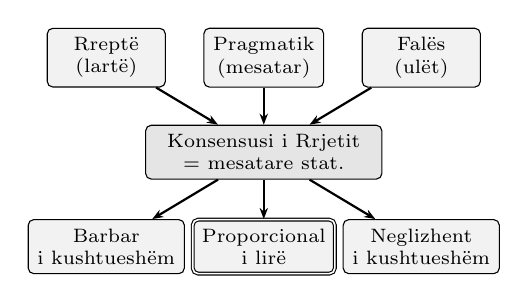
\begin{tikzpicture}[
    person/.style={draw, rounded corners=2pt, minimum width=1.5cm, minimum height=0.5cm, align=center, font=\scriptsize, fill=black!5},
    arr/.style={-{Stealth[length=4pt]}, thick}
]
\node[person] (a) at (-2,0) {Rreptë\\(lartë)};
\node[person] (b) at (0,0) {Pragmatik\\(mesatar)};
\node[person] (c) at (2,0) {Falës\\(ulët)};
\node[person, fill=black!10, minimum width=3cm] (cons) at (0,-1.2) {Konsensusi i Rrjetit\\= mesatare stat.};
\node[person] (exp) at (-2,-2.4) {Barbar\\i kushtueshëm};
\node[person, double] (prop) at (0,-2.4) {Proporcional\\i lirë};
\node[person] (neg) at (2,-2.4) {Neglizhent\\i kushtueshëm};

\draw[arr] (a) -- (cons);
\draw[arr] (b) -- (cons);
\draw[arr] (c) -- (cons);
\draw[arr] (cons) -- (exp);
\draw[arr] (cons) -- (prop);
\draw[arr] (cons) -- (neg);
\end{tikzpicture}
\caption{Konsensusi emergjent nga pragjet individuale të kënaqësisë.}
\label{fig:consensus}
\end{figure}

\subsection{Kalibrimi i Ndëshkimit}

Çdo Mbajtës DID deklaron publikisht përgjigjet ndaj kategorive specifike të sjelljes së keqe. Deklaratat në mënyrë joproporcionale të ashpra ose të buta tërheqin sinjale negative reputacioni. Deklaratat proporcionale pranohen pa fërkim---një sistem ndëshkimi vetëkalibrues.

Deklaratat e konsensusit janë vetë subjekt i zbulimit të hipokrizisë: zotimi deklarativ ndaj një pozicioni konsensusi ndërsa sillet në mënyrë të mospërputhshme përbën një shkelje reputacioni më të rëndë se vetë devijimi themelor, sepse tregon mashtrim të qëllimshëm.

\subsection{Delegimi}

Të gjitha aktivitetet brenda një DID---me një përjashtim---mund t'i delegohen një DID-i tjetër. \textbf{Roli i Subjektit---DID-i sjellja e të cilit është objekt i pretendimit---nuk mund të delegohet; ai është i lidhur në mënyrë të patransferueshme me mbajtësin e identitetit të cilit i referohet pretendimi.} Rolet e tjera aktive---Lëshuesi, Autoriteti, Dëshmitari, Verifikuesi---mund t'i transferohen një DID-i të caktuar përfaqësuesi, qoftë për verifikim, paraqitje pretendimi, pjesëmarrje në konsensus ose zgjidhje mosmarrëveshjesh. Delegimi është i revokueshëm në çdo kohë. Kjo mundëson specializim (p.sh., shërbime profesionale verifikimi) ndërsa Mbajtësi ruan kontrollin dhe përgjegjësinë përfundimtare. Delegimi zbatohet në të gjithë sistemin dhe është thelbësor për shkallëzueshmërinë.

\subsection{Nga Morali Individual te Kontrata Shoqërore Emergjente}

Politika e deklaruar e çdo DID-i përfaqëson një formalizim të moralit individual: çfarë e konsideron Mbajtësi të pranueshme, si u përgjigjet sjelljeve specifike, çfarë kërkon nga palët e tjera. Këto politika nuk imponohen nga një projektues sistemi---ato zgjidhen nga çdo pjesëmarrës dhe shprehen në formë të lexueshme nga makina.

Ky formalizim mundëson një shfaqje trefazore. Së pari, morali individual kodohet si \textbf{politikë}---një grup rregullash të deklaruara, pragjesh dhe funksionesh përgjigjeje që DID-i zotohet t'i ndjekë. Së dyti, agregati i të gjitha politikave nëpër rrjet prodhon \textbf{etikë emergjente}---norma të vëzhgueshme statistikisht që asnjë pjesëmarrës i vetëm nuk i projektoi por që lindin nga bashkëveprimi i mijëra pozicioneve individuale morale~\cite{durkheim1893}. Së treti, kjo etikë emergjente, e shprehur si norma të përbashkëta sjelljeje të zbatuara përmes sinjaleve dypalëshe të çmimit, përbën një \textbf{kontratë shoqërore të matshme}---jo një konstrukt teorik që askush nuk e nënshkroi~\cite{rawls1971}, por një grup rregullash empirikisht të vëzhgueshme të mbështetura nga sjellje aktuale.

Ky proces pasqyron gjetjet nga teoria e themeleve morale~\cite{haidt2012}: morali njerëzor është intuitiv, pluralist dhe kulturalisht i ndryshueshëm. RSN nuk kërkon konsensus moral si hyrje; ai prodhon konsensus sjelljeje si dalje. Kontrata shoqërore që rezulton nuk është statike---ajo evoluon ndërsa pjesëmarrësit bashkohen, largohen dhe rregullojnë politikat e tyre në përgjigje të reagimeve të rrjetit. Ndryshe nga teoria klasike e kontratës shoqërore, kjo kontratë është e revokueshme, e vëzhgueshme dhe e zbatueshme pa një sovran.

% ============================================================
% 8. ECONOMIC MODEL
% ============================================================
\section{Modeli Ekonomik}

Seksionet paraprake përshkruan një mjet---mekanizmat e verifikimit të RSN, strukturën e kostos dhe konsensusin emergjent. Ky seksion përshkruan një metodologji për zbatimin e këtij mjeti në tranzicionin fiskal dhe të qeverisjes. Mjeti është i qëllimit të përgjithshëm; metodologjia më poshtë është një zbatim i mundshëm.

\subsection{Struktura e Stimujve}

Reputacioni si kapital krijon stimuj të drejtpërdrejtë për sjellje të ndershme. Në funksionimin normal, pjesëmarrësit ndërtojnë reputacion natyrshëm përmes transaksioneve të përditshme dhe zotimeve të përmbushura. Shpenzimi kryesor bëhet për pretendime \emph{negative}---regjistrimi i dëmit të bërë nga të tjerët. Kjo asimetri stimulon sjellje të dobishme dhe të besueshme: të qenit i ndershëm nuk kushton asgjë shtesë, ndërsa të qenit i dëmshëm krijon një gjurmë të dokumentuar që të tjerët do të paguajnë për ta ruajtur. Hipokrizia---deklarimi i rregullave pa i ndjekur ato---është mënyra më e kushtueshme e dështimit, sepse tregon mashtrim të qëllimshëm.

\subsection{Sistemi Fiskal Paralel}

Tre komponentë mundësojnë presion konkurrues: (1)~\textbf{Taksë e Thjeshtë}---një normë e vetme proporcionale pa përjashtime, fillimisht marxhinalisht nën normën ekzistuese efektive; (2)~\textbf{Regjistrimi Elektronik i Shpenzimeve (ESR)}---duke përmbysur modelin çek EET në mënyrë që qytetarët të mbikëqyrin shpenzimet e shtetit; (3)~\textbf{Ndarja e Taksës e Drejtuar nga Qytetari}---duke filluar me pak për qind në vitin e parë dhe duke arritur, pas një dekade, kudo nga shifra dyshifrore të ulëta deri në një migrim të plotë drejt një sistemi të drejtuar nga qytetari, në varësi të normës së miratimit. Tempoja aktuale varet nga shpejtësia me të cilën shfaqen alternativat e tregut të lirë ndaj shërbimeve shtetërore dhe nga gatishmëria e shtetit për të bashkëpunuar me tranzicionin; funksioni i kohës nuk ka pse të jetë linear, dhe nuk ka arsye për të vendosur një kufi të sipërm se ku mund të arrijë miratimi përfundimisht.

% ============================================================
% 9. MIGRATION PATH
% ============================================================
\section{Rruga e Migrimit}

Migrimi vazhdon nëpër tri faza (Fig.~\ref{fig:migration}): \textbf{Faza~1: Mbivendosja} (RSN si shtresë informative, shteti është ofruesi i vetëm), \textbf{Faza~2: Konkurrenca} (RSN ofron alternativa funksionale, përdorim i sistemit të dyfishtë) dhe \textbf{Faza~3: Tranzicioni} (RSN i tejkalon ekuivalentët shtetërorë, migrim vullnetar). Tranzicioni është i kthyeshëm në çdo fazë.

\begin{figure}[ht]
\centering
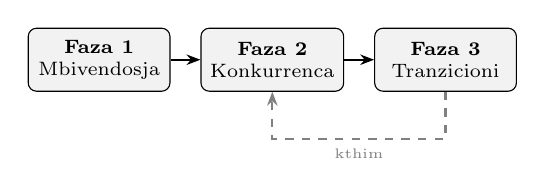
\begin{tikzpicture}[
    phase/.style={draw, rounded corners=3pt, minimum width=1.8cm, minimum height=0.8cm, align=center, font=\scriptsize, fill=black!5},
    arr/.style={-{Stealth[length=5pt]}, thick}
]
\node[phase] (p1) at (0,0) {\textbf{Faza 1}\\Mbivendosja};
\node[phase] (p2) at (2.2,0) {\textbf{Faza 2}\\Konkurrenca};
\node[phase] (p3) at (4.4,0) {\textbf{Faza 3}\\Tranzicioni};

\draw[arr] (p1) -- (p2);
\draw[arr] (p2) -- (p3);
\draw[arr, dashed, gray] (p3.south) -- ++(0,-0.6) -| node[below,font=\tiny,pos=0.25] {kthim} (p2.south);
\end{tikzpicture}
\caption{Migrimi trefazor---i kthyeshëm në çdo fazë.}
\label{fig:migration}
\end{figure}

Mekanizmi kryesor i presionit është fiskal: kur taksapaguesit e kushtëzuar arrijnë një ``pakicë ekonomikisht të konsiderueshme $X$''---një grup mjaftueshëm i madh sa që represioni kundër tij shkakton dëm ekonomik jotrivial dhe mosbindja civile bëhet një kërcënim i besueshëm---shteti hyn në negocim. Për ilustrim, përdorim $X \approx 15\%$ të PBB-së, por pragu aktual varet nga ekonomia specifike.

% ============================================================
% 10. SECURITY ANALYSIS
% ============================================================
\section{Analiza e Sigurisë}

Ne shqyrtojmë pesë kategori kundërshtarësh: aktorë të këqij individualë, grupe të organizuara, kundërshtarë korporativë, kundërshtarë në nivel shteti dhe kundërshtarë në nivel protokolli.

\textbf{Rezistenca ndaj Sybil}~\cite{douceur2002}. Ndërtimi i reputacionit kërkon bashkëveprim të vazhdueshëm dhe të verifikueshëm. Kostoja e një sulmi të suksesshëm Sybil shkallëzohet linearisht me identitetet e rreme dhe kuadratikisht me nivelin e reputacionit objektiv. Vënia në funksion e shumë DID-ve paralelisht është e mundur por e kushtueshme nga dizajni---çdo identitet duhet të akumulojë në mënyrë të pavarur reputacion përmes aktivitetit të vërtetë. Në shoqëritë e lira kjo kosto pengon abuzimin e rastësishëm; në diktatura, DID-të paralele bëhen një mjet mbijetese që mundëson rezistencë të ndarë në kompartimente, koordinim të nëndheshëm dhe lundrim më të sigurt në tregun e zi.

\textbf{Mbrojtja ndaj marrëveshjeve të fshehta.} Modelet e miratimit të ndërsjellë mes grupeve të mbyllura janë të zbulueshme përmes analizës së grafit shoqëror. Funksionet e grumbullimit të reputacionit i zbresin pretendimet nga burime të grupuara ngushtë.

\textbf{Kundërshtari në nivel shteti.} Rrugëzimi onion, mungesa e infrastrukturës së centralizuar dhe shpërndarja e rolit të Verifikuesit nëpër bazën e pjesëmarrësve sigurojnë që shtypja të kërkojë masa joproporcionale me çdo përfitim.

\textbf{Privatësia kundrejt llogaridhënies.} Pseudonimiteti---një terren i mesëm mes anonimitetit dhe zbulimit të identitetit---u lejon DID-ve të akumulojnë reputacion domethënës pa zbuluar identitetin real të Mbajtësit.

% ============================================================
% 11. PRIVACY
% ============================================================
\section{Konsiderata të Privatësisë}

Modeli i privatësisë së RSN ndërtohet mbi pseudonimitet. Mbajtësi kontrollon zbulimin e identitetit: minimal (pseudonim i pastër), selektiv (kredenciale specifike të lidhura) ose i plotë (identitet ligjor i shoqëruar). Pretendimet e publikuara janë të përhershme---sistemi mbështet korrigjimin kontekstual por jo fshirjen. Një Mbajtës mund të braktisë një DID të kompromentuar dhe të fillojë nga e para, duke humbur reputacionin e akumuluar.

% ============================================================
% 12. RELATED WORK
% ============================================================
\section{Punë e Ngjashme}

Specifikimi W3C DID Core~\cite{did2022} dhe Ceramic Network~\cite{ceramic2023} ofrojnë themelin e identitetit. EigenTrust~\cite{kamvar2003} demonstroi grumbullimin e shpërndarë të reputacionit pa autoritet qendror. SBT-të~\cite{weyl2022} prezantuan tokenat shoqërorë të patransferueshëm. RSN dallon në theksimin e tij mbi koston ekonomike si filtër cilësie dhe në mekanizmin e tij për çmimin e radikalizmit.

DAO-t~\cite{buterin2014} dhe votimi kuadratik~\cite{buterin2019} demonstruan realizueshmërinë e qeverisjes së decentralizuar. RSN e nxjerr konsensusin nga negocimet dypalëshe të çmimit sesa nga votimi.

Propozimi mbështetet në teorinë anarko-kapitaliste~\cite{rothbard1973,hoppe2001} për ofrimin privat të shërbimeve por largohet në dy aspekte kritike: ai projekton për inatin dhe impulset ndëshkuese sesa të supozojë racionalitet, dhe propozon tranzicion gradual sesa revolucion. Koncepti i kontratave shoqërore emergjente ka paraardhës në teorinë e Hayek-ut për rendin spontan~\cite{hayek1973}.

\textbf{Anarko-agorizmi.} RSN ndan terren të konsiderueshëm të përbashkët me kundërekonominë agoriste~\cite{konkin2006}---veçanërisht theksimin mbi ndërtimin e institucioneve paralele dhe shkëmbimin vullnetar. Megjithatë, agorizmi priret të supozojë interesin racional të vetes si mekanizëm koordinimi të mjaftueshëm dhe shpesh i mungon një rrugë konkrete migrimi nga strukturat ekzistuese shtetërore. RSN përfshin në mënyrë të qartë prirjet joracionale të sjelljes dhe ofron një mekanizëm presioni fiskal për tranzicion gradual.

\textbf{Meritokracia.} RSN mund të përfaqësojë një përshkrim të parë funksional se si meritokracia~\cite{young1958} mund të lindë si veti sistemike sesa si slogan. Sistemet tradicionale meritokratike dështojnë sepse kërkojnë një autoritet qendror për të përcaktuar dhe zbatuar ``meritën''. Në RSN, merita lind nga vlerësimet dypalëshe: ata që ofrojnë vlerë akumulojnë reputacion; asnjë komitet nuk vendos se kush ka meritë.

\textbf{Prona si privilegj.} RSN largohet thelbësisht nga trajtimet anarko-kapitaliste dhe të shkollës austriake të të drejtave të pronës si natyrore dhe absolute. Në kornizën e RSN, prona është një \emph{privilegj}---një njohje shoqërore që mundet, në raste ekstreme, të tërhiqet nga komuniteti kur një pjesëmarrës shkel thelbësisht normat e përbashkëta (tradhtia, refuzimi për të mbrojtur komunitetin në krizë ekzistenciale, shfrytëzimi sistematik). Ky nuk është shpronësim shtetëror por një tërheqje e njohjes shoqërore nga rrjeti i marrëdhënieve dypalëshe.

% ============================================================
% 13. LIMITATIONS
% ============================================================
\section{Diskutimi dhe Kufizimet}

\textbf{Nisja e ftohtë.} Vlera e RSN varet nga efektet e rrjetit; miratuesit e hershëm përballen me vlerë të kufizuar derisa pjesëmarrja të arrijë një prag. Megjithatë, edhe nga fazat e hershme, rrjeti DID shërben si burim i dobishëm informacioni plotësues. Vlerësimi i hershëm i reputacionit dhe vlerësimi i autoritetit pritet të zhvillohen gradualisht me sofistikim në rritje.

\textbf{Anti-parazitizmi dhe kontrolli i qasjes.} DID-të objektiv mund të vendosin tarifa të shkallëzuara dhe kufizime qasjeje mbi pyetësimet nga DID me reputacion të ulët. Kjo nuk është binare por një shkallë e vazhdueshme: sa më pak reputacion të ketë një DID pyetës, aq më pak informacion merr, aq më gjatë pret dhe aq më shumë paguan. Ky mekanizëm stimulon pjesëmarrjen e vërtetë mbi konsumimin pasiv.

\textbf{Pabarazia e qasjes.} Kostoja e publikimit të pretendimeve mund të filtrojë ankesat legjitime nga pjesëmarrësit ekonomikisht të disavantazhuar. Zbutja: çdo pjesëmarrës shërben njëkohësisht si verifikues i mundshëm (ose e delegon këtë rol) dhe fiton tarifa verifikimi. Përgjatë një horizonti të mjaftueshëm kohor, një pjesëmarrës joradikal duhet t'i afrohet neutralitetit financiar---të ardhurat nga verifikimi kompensojnë përafërsisht kostot e publikimit. Kjo është një pritje statistikore, jo një garanci.

\textbf{Pabarazia e reputacionit.} Miratuesit e hershëm akumulojnë avantazhe që mund të krijojnë barriera për vonardhurit. Megjithatë, vlerësimi i reputacionit kryhet nga ofrues të palëve të treta që mund të zgjedhin të zbusin avantazhin e lëvizësit të parë përmes algoritmeve të tyre të grumbullimit. Të qenit i pari me reputacion të mirë është një avantazh legjitim krahasues ekonomik---dhe kjo është nga dizajni.

\textbf{Pyetje të hapura.} Funksionet optimale të kostos, standardet e grumbullimit, qeverisja e protokollit dhe bashkëveprimi me të dhëna sintetike të reputacionit të gjeneruara nga IA mbeten fusha për punë të ardhshme.

Ky punim nuk pretendon se RSN do të prodhojë rezultate optimale në të gjitha rrethanat. Ai pretendon se RSN përfaqëson një alternativë \emph{të realizueshme}---teknikisht të zbatueshme, ekonomikisht vetëmbajtëse dhe shoqërisht të përputhshme me prirjet e sjelljes njerëzore ashtu siç janë në të vërtetë.

% ============================================================
% 14. CONCLUSION
% ============================================================
\section{Përfundim}

Ky punim ka paraqitur Rrjetin Shoqëror të Reputacionit, një protokoll të decentralizuar që mundëson shkëmbim reputacioni pseudonim dhe të verifikueshëm. Parimi i Radikalizmit të Kushtueshëm siguron që pretendimet mashtruese të çmohen jashtë tregut pa censurë. Rruga e propozuar e migrimit mundëson tranzicion gradual dhe të kthyeshëm nga institucionet ekzistuese. Dizajni përfshin natyrën njerëzore ashtu siç është---duke përfshirë smiritetin, inatin dhe dëshirën për kënaqësi ndëshkuese---sesa të kërkojë transformim ideologjik. Rezultati nuk është utopi por një sistem ku drejtësia është e qasshme, reputacioni fitohet dhe kostoja e sjelljes së keqe mbahet nga pala që e shkaktoi atë.

% ============================================================
% REFERENCES
% ============================================================
\bibliography{references}

\end{document}
